\documentclass[final]{cvpr}

% NOTE(brendan):
% https://tex.stackexchange.com/questions/398223/tikz-gives-error-command-everyshipouthook-already-defined/398269
\makeatletter
\@namedef{ver@everyshi.sty}{}
\makeatother
\usepackage{tikz}
\usepackage{times}
\usepackage{epsfig}
\usepackage{graphicx}
\usepackage{amsmath}
\usepackage{amssymb}

% Include other packages here, before hyperref.
\usepackage[normalem]{ulem}
\usepackage{siunitx}

% NOTE(brendan): my packages
\usepackage{bbm}  % for \mathbbm{1}
\usepackage{bm}  % for more powerful bold symbols https://tex.stackexchange.com/a/596
\usepackage{caption}
\captionsetup[table]{skip=5pt}  % space between table and caption https://tex.stackexchange.com/a/2836
\usepackage{booktabs}
\usepackage{pifont}  % for dingbats checkmark and xmark

% If you comment hyperref and then uncomment it, you should delete
% egpaper.aux before re-running latex.  (Or just hit 'q' on the first latex
% run, let it finish, and you should be clear).
\usepackage[pagebackref=true,breaklinks=true,letterpaper=true,colorlinks,bookmarks=false]{hyperref}

% NOTE(brendan): my macros
% https://tex.stackexchange.com/a/217624
\makeatletter
\newcommand*{\transpose}{%
	{\mathpalette\@transpose{}}%
}
\newcommand*{\@transpose}[2]{%
	% #1: math style
	% #2: unused
	\raisebox{\depth}{$\m@th#1\intercal$}%
}
\makeatother

% \makeatletter                  % You do not need to write [htpb] all the time
% \renewcommand\fps@figure{htbp} %
% \renewcommand\fps@table{htbp}  %
% \makeatother                   %

\def\cvprPaperID{3473} % *** Enter the CVPR Paper ID here
\def\confYear{CVPR 2021}

\newcommand{\myparagraph}[1]{\textbf{#1 ---}}


\begin{document}

\title{Building and Analyzing a 2D DiffuserCam at Home}

\author{Brendan Duke}

\maketitle

\section{Experimental Setup}

I converted a PiCam V2 to build my DiffuserCam.
I had to remove the lens, since DiffuserCam is a lensless camera.
Furthermore I had to remove the IR filter and plastic housing for the camera
from the sensor (Fig.~\ref{fig:board-filter-sensor}).
This is because the 2mm focal length of my diffuser,
double-sided tape, was smaller than the thickness of the camera housing itself.
I instead used cardboard as a separating material to place the diffuser at the
correct 2mm focal length from the sensor.
I determined the focal length by analyzing the full width at half maximum
(FWHM)

I used a cement mixing tray (Fig.~\ref{fig:experimental-setup}) to provide
a dark environment for calibrating the DiffuserCam.
When taking photos I covered the mixing tray completely so that a single white
LED (also in the tray) was the only light source illuminating the camera
sensor.
I created a pinhole aperture out of cardboard and placed it in front of the LED
to make the LED more closely resemble a point source.
With the tray covered, I read images from the camera in real time.
I adjusted the voltage applied to the LED so that the image pixels did not
saturate, which would violate the linearity assumption made about the point
spread function (PSF) in the reconstruction optimization.
I used the same experimental setup for taking photos of objects to reconstruct.
When reconstructing objects displayed on my phone I adjusted the PiCam exposure
time in order to prevent pixel saturation.


\begin{figure*}[t]
	\centering
	\includegraphics[width=1.0\linewidth]{images/experimental-setup}
	\caption{\label{fig:experimental-setup}
		The experimental setup used to conduct calibration and collect images.
		I used the power supply (bottom) to adjust the brightness of the LED in order to prevent image saturation.}

\end{figure*}



\begin{figure}[t]
	\centering
	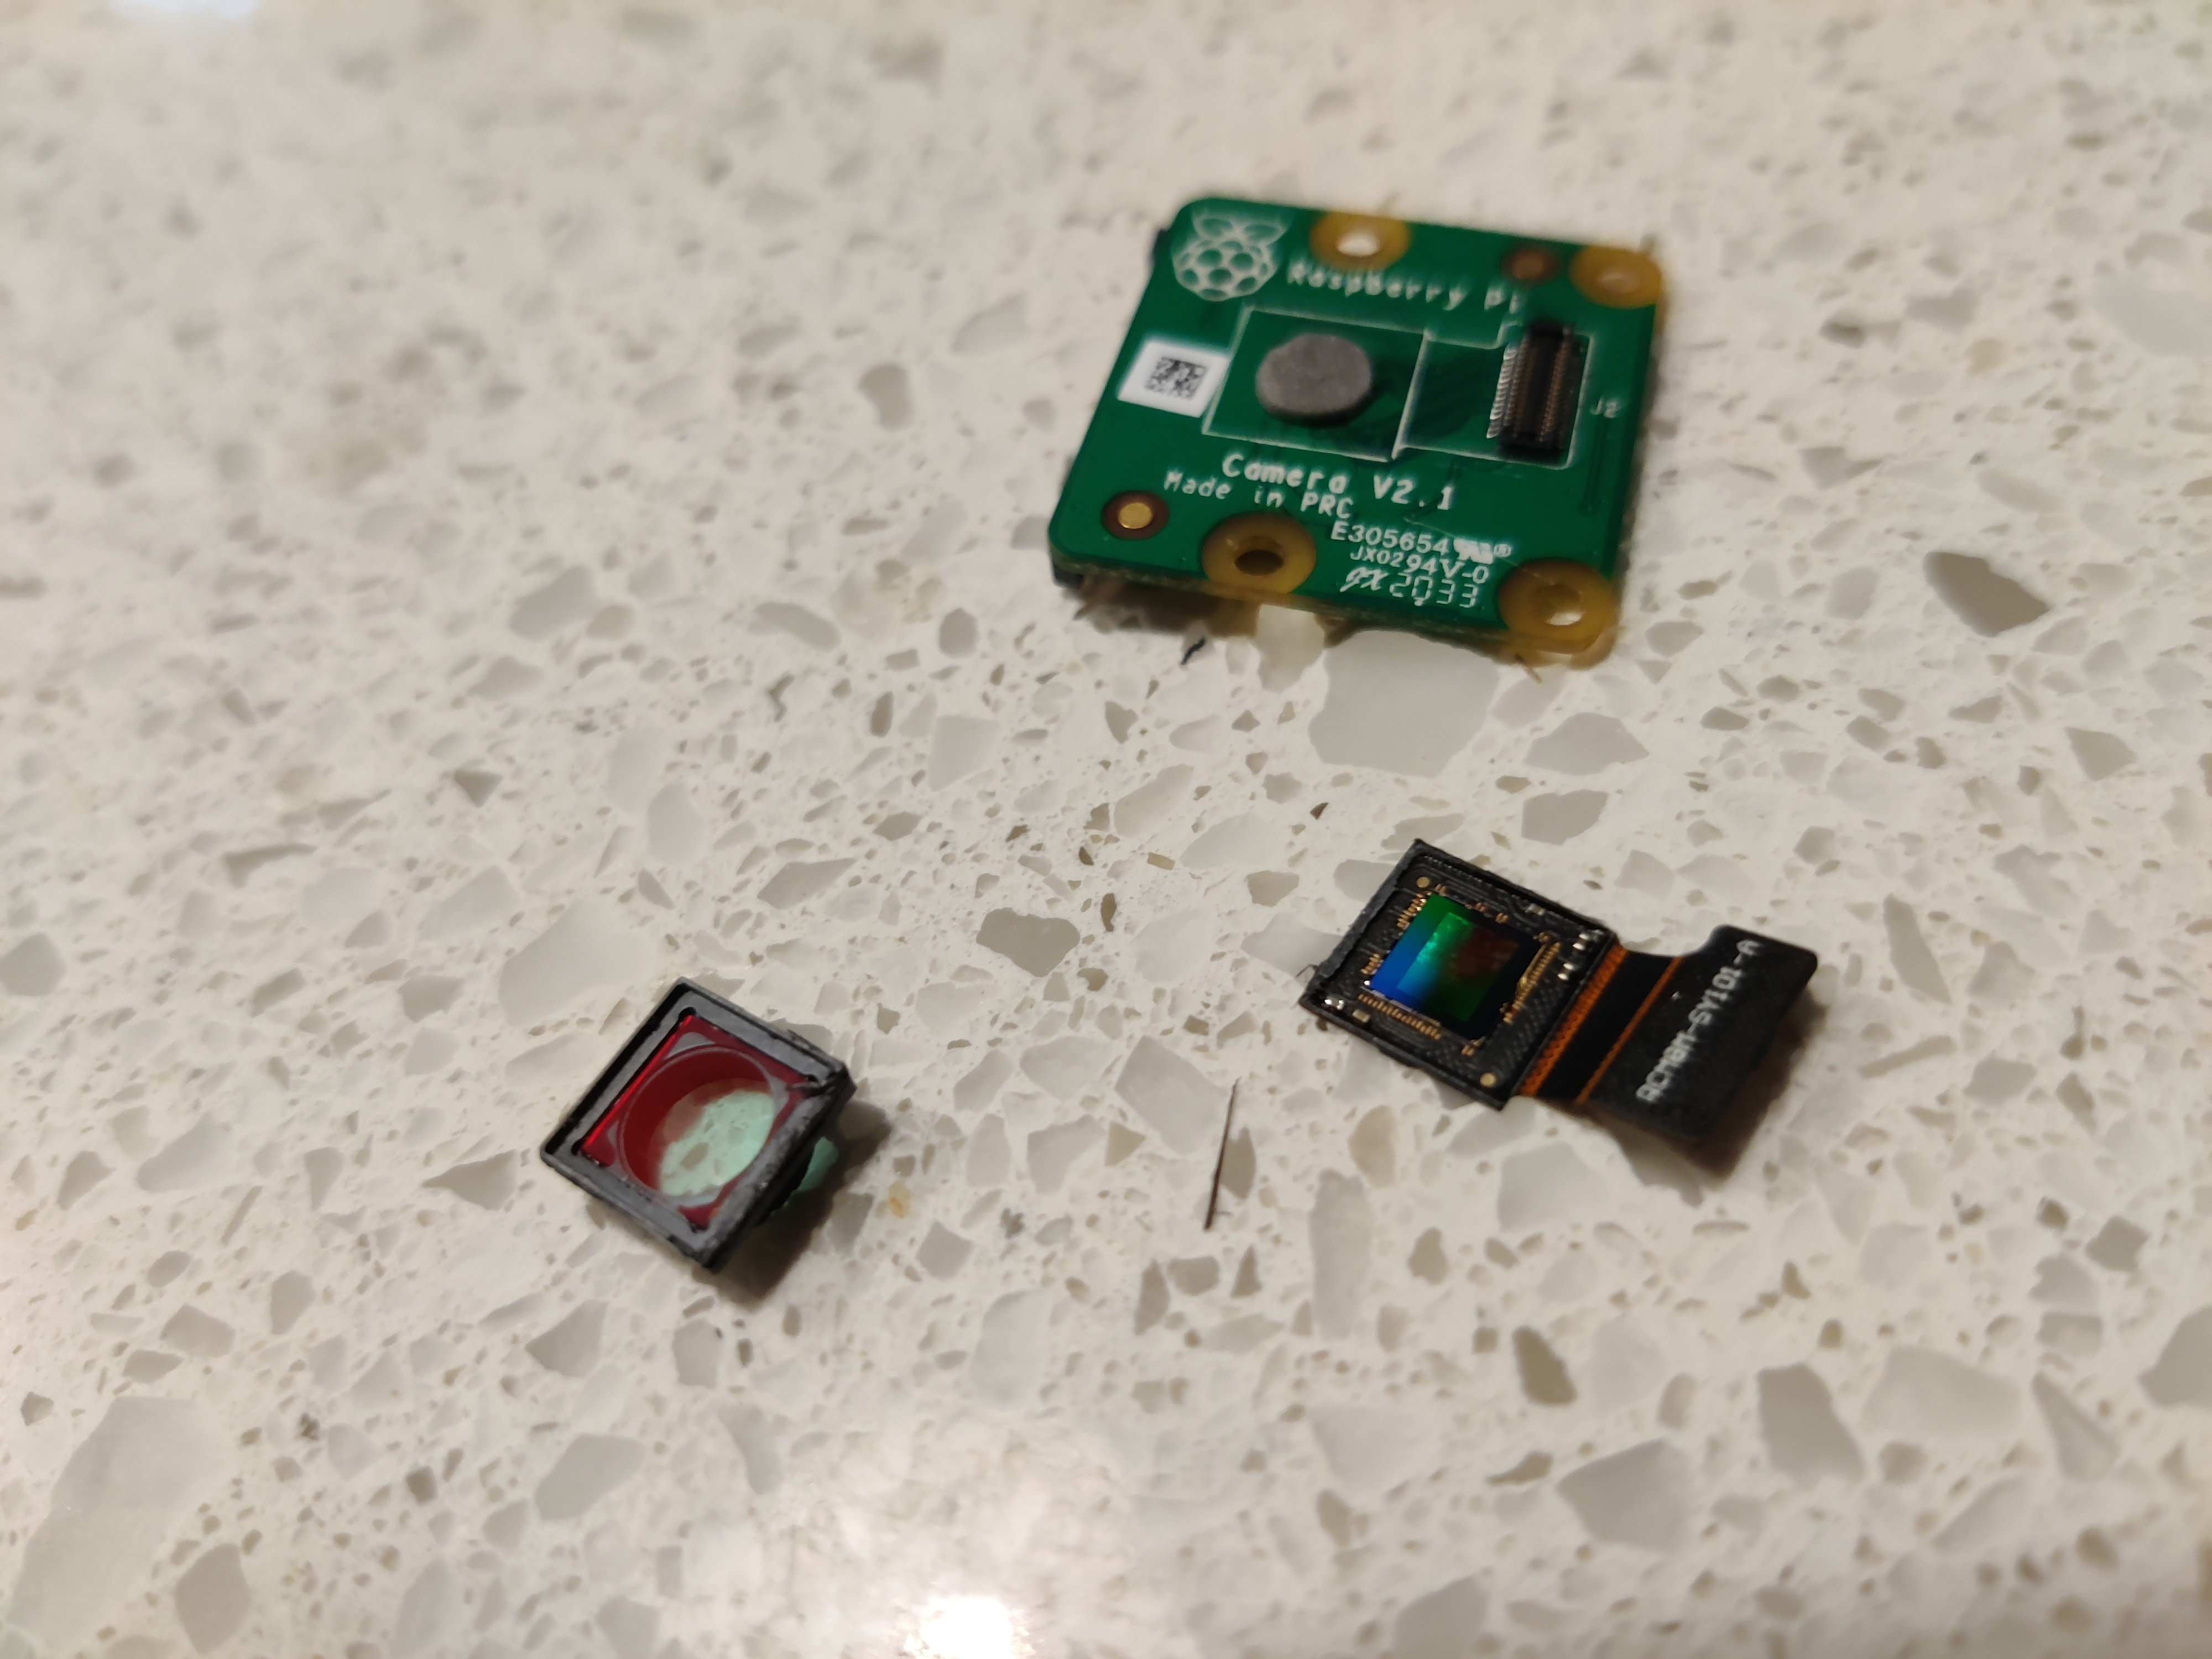
\includegraphics[width=1.0\linewidth]{images/board-filter-sensor}
	\caption{\label{fig:board-filter-sensor}
		The Raspberry PiCam V2 camera board, IR filter, and sensor disassembled to create a DiffuserCam.}
\end{figure}



\section{Results}



\begin{figure}[t]
	\centering
	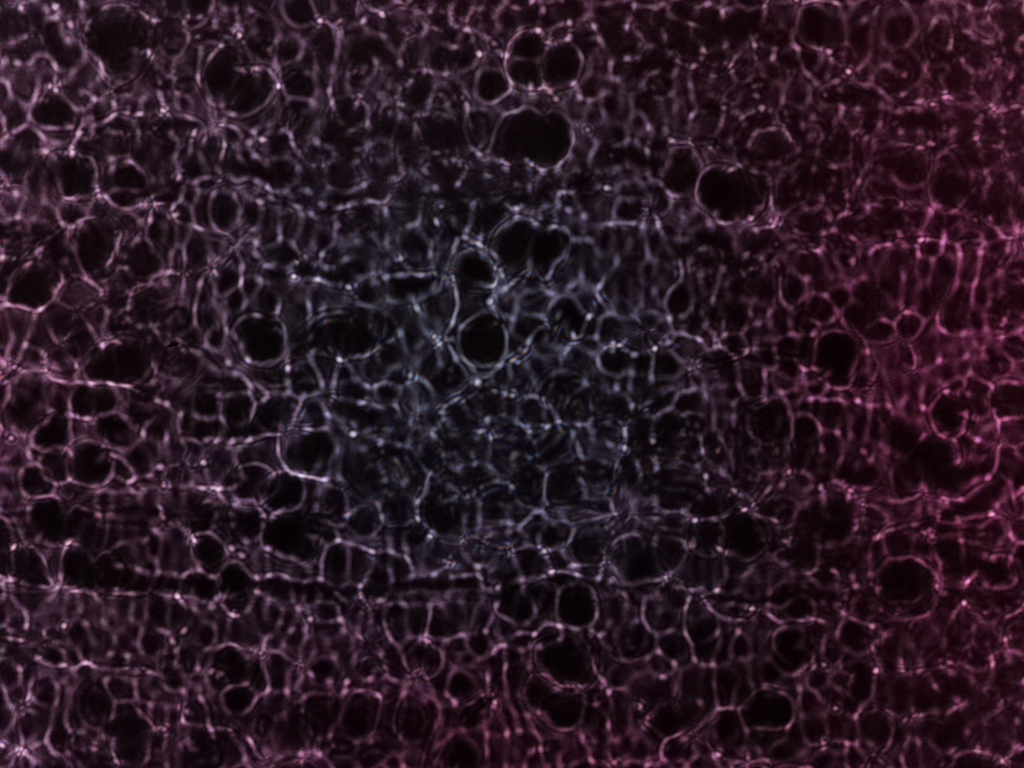
\includegraphics[width=1.0\linewidth]{images/caustic}
	\caption{\label{fig:caustic}
		Caustics produced by applying~\num{2.5}V to the LED\@.
		To form this image the sensor was separated by about~\num{2}mm
		of separating material (cardboard) from the diffuser (double-sided tape).
		Qualitatively, the focal length of the diffuser was about~\num{2}mm.}
\end{figure}


\begin{figure}[t]
	\centering
	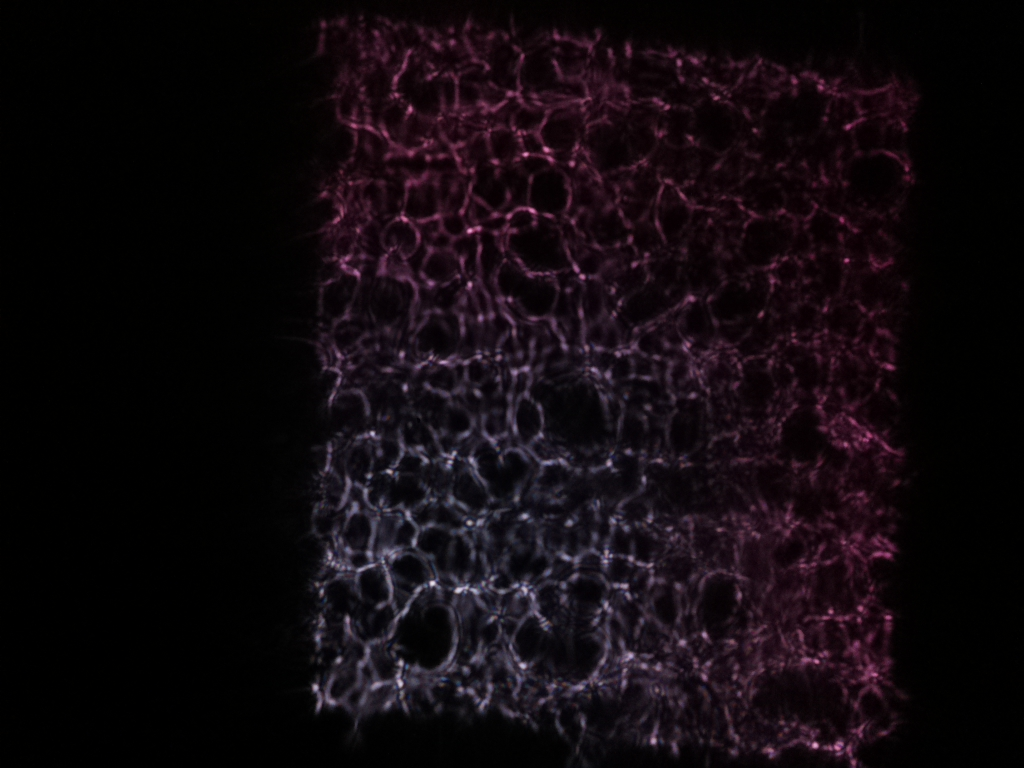
\includegraphics[width=1.0\linewidth]{images/caustic-with-aperture}
	\caption{\label{fig:caustic-with-aperture}
		Caustics produced by applying~\num{2.5}V to the LED\@.
		Here an aperture made from black tape creates a black border
		around the caustic pattern.
		Without the aperture single-shot calibration would not be
		possible, because new caustics would come into view when the
		point source moves.}
\end{figure}


\begin{figure*}[t]
	\centering
	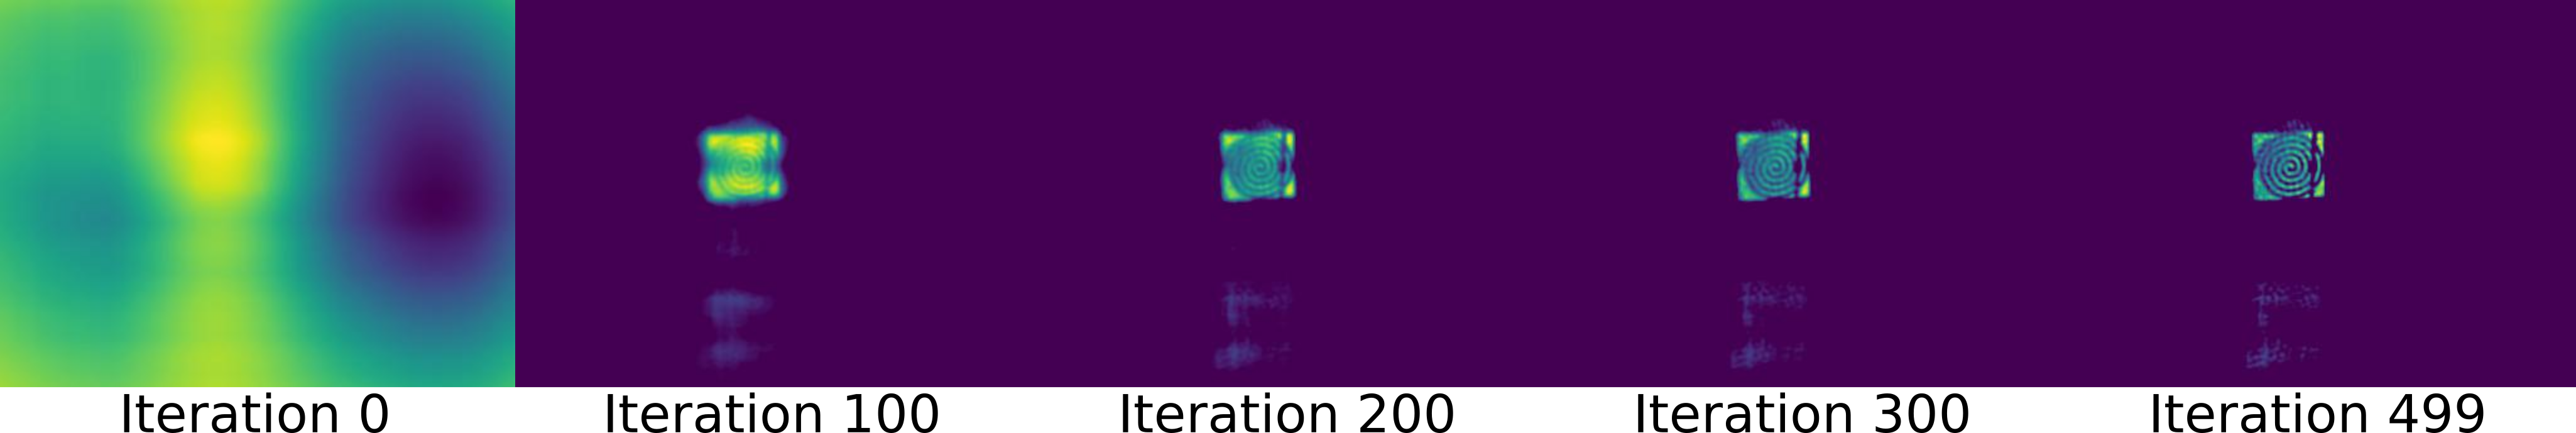
\includegraphics[width=1.0\linewidth]{images/gd-spiral-reconstruction-500iters}
	\caption{\label{fig:gd-spiral-reconstruction-500iters}
		Gradient descent (GD) reconstruction of a spiral image
		displayed on a cell phone in an otherwise dark environment.
		The update step uses FISTA~\cite{beck2009fast} and a
		non-negativity projection.
		GD reconstructs the spiral image clearly after about 200 epochs.
		The bar on the right side of the spiral is an occlusion from a
		stand holding up the cell phone.}
\end{figure*}









\par\vfill\par

\clearpage
% ---- Bibliography ----
%
% BibTeX users should specify bibliography style 'splncs04'.
% References will then be sorted and formatted in the correct style.
%
{\small
	\bibliographystyle{ieee_fullname}
	\bibliography{report}
}

\clearpage

\end{document}
